\documentclass{ieeeaccess}
\usepackage{cite}
\usepackage{amsmath,amssymb,amsfonts}
\usepackage{algorithmic}
\usepackage{graphicx}
\usepackage{textcomp}
\usepackage{multirow}
\usepackage[colorlinks,
linkcolor=black,
anchorcolor=black,
citecolor=blue]{hyperref}
\usepackage[numbers]{natbib}
\usepackage{bm}

\def\BibTeX{{\rm B\kern-.05em{\sc i\kern-.025em b}\kern-.08em
    T\kern-.1667em\lower.7ex\hbox{E}\kern-.125emX}}
\begin{document}
\history{Date of publication xxxx 00, 0000, date of current version 2019 09, 02.}
\doi{10.1109/ACCESS.2019.DOI}

\title{Transformer Based Memory Network for Sentiment Analysis of Web Comments}
\author{
	\uppercase{Ming Jiang}, 
	\IEEEmembership{Member, IEEE}, 
	\uppercase{Junlei Wu, 
		and Min Zhang}.}
\address{Xiasha Higher Education Zone, Hangzhou, 310018, Zhejiang Province, People's Republic of China}

\tfootnote{This work is supported by Zhejiang Provincial Technical Plan Project (No. 2018C03039, 2018C03052).}

\corresp{Corresponding author: Junlei Wu (e-mail: 171050047@hdu.edu.cn).}

\begin{abstract}
With the rapid development of edge devices and wireless technologies, a large amount of comments has been generated in the network. Therefore, the sentiment feature extraction of web comments is of great significance, and aspect-based sentiment analysis (\textit{ABSA}) is useful to retrieval the sentiment feature from web comments. Now, context-dependent sentiment feature is obtained by widely using long short-term memory (\textit{LSTM}) or Gated Recurrent Unit (\textit{GRU}) network, and target vector is usually replaced by average target vector. However, web comments has become increasingly complex and feature extraction with \textit{LSTM} or \textit{GRU} might cause the loss of key sentiment information. Meanwhile, average target vector might be wrong target feature. To correct drawbacks of the old method, a new Transformer (a new neural network architecture based on self-attention mechanism) based memory network (\textit{TF-MN}), is introduced. In \textit{TF-MN}, the task is migrated into question answering process in which context, question and memory module is modified optimally. The comment is encoded by Transformer in context module, question module transfer target into sentiment question, memory module eliminates the effect of unrelated words by several extractions. The result of the experiment proves that our model reaches better accuary than the state-of-the-art model.
\end{abstract}

\begin{keywords}
ABSA, Transformer, Memory Network, Web Comments
\end{keywords}

\titlepgskip=-15pt

\maketitle

\section{Introduction}
\label{sec:introduction}
\PARstart{I}{n} the future, there will be billions of devices connected to the Internet, and we will be surrounded by data. So faster and more reliable data processing will become critical. In recent years, the integration and centralized nature of cloud computing has proven to be cost-effective and flexible, but the rise of the Internet of Things and mobile computing has put a lot of pressure on network bandwidth. Ultimately, not all smart devices need to run with cloud computing. In some cases, round-trip transmission of data can be avoided. For example, web comments contains a large amount of text and images, and transferring this data requires a lot of network resources. Using edge computing technology, we can store this data in a nearby server, then extract key information from the data and pass it back to the server. The emotional information contained in the web comments is a very important feature, and it is necessary to extract it. In this article, we mainly conduct sentiment analysis on the web comments of Weibo.

As one of the most important mobile social applications, Weibo contains entertainment, social, marketing, food and so on \cite{DBLP:conf/IEEEcit/ChenLZW16}. It has gradually evolved from a social demand that satisfies people’s “we$  $ak relationship” to a popular public opinion platform, becoming one of the most important realtime information sources and the center of spreading public opinion. Viewpoints and proposals in Weibo are universal and adaptive due to large amounts of users along with the differences of their standpoints and knowledge they have. By performing sentiment analysis on the content published by Weibo users, it can restore the real emotions of users as much as possible, help people to get hot topics in time, help control the direction of public opinion, and help to analyze product reviews. This sentiment analysis technology not only assists users in optimizing their purchasing decisions, but also helps them to self-improve, improve market competitiveness, and accurately discover and exploit the hidden business and social values in Weibo.

Weibo sentiment analysis refers to judging the emotional tendency by analyzing and mining subjective information in Weibo. At present, there are many studies on the emotional analysis of Weibo in China. According to the granularity, it can be divided into fine-grained sentiment analysis and coarse-grained sentiment analysis. The coarse-grained sentiment analysis is mainly based on the text level and the sentence level, and only the emotional words are considered in the analysis process, and the emotions of the evaluation object and its attributes are not considered; Fine-grained sentiment analysis generally refers to lexical-level sentiment analysis.

In this paper, we use aspect level sentiment analysis(ABSA), a fine-grained sentiment analysis technology, to process Weibo texts. A piece of Weibo text may contains many aspects, each of which expresses a variety of emotions. For example, the text, “Nice Service but the food was too bad!”, expresses the emotions of two different goals. With the approach of aspect level sentiment analysis, we can analyze the opinions and emotions expressed by Weibo in a more fine-grained manner. As to the above instance, we analyze the emotions to be expressed in this text from two aspects. The polarity is positive when target is “service”, but it turns negative if “food” is seen as target. This hierarchical analysis method is very effective for digging deep into the emotions expressed by a piece of text.

In terms of sentiment classification, whether it is coarse-grained or fine-grained sentiment analysis, the methods used can be divided into three categories, supervised machine learning methods, unsupervised sentiment analysis methods, and semi-supervised sentiment analysis methods.

Supervised machine learning methods perform supervised training and testing through classifiers by selecting emotional classification features such as emotional words. The milestone is that Pang et al. applied three representative classifiers (support vector machine SVM, naive Bayes NB, maximum entropy ME) to classify the text emotionally~\cite{DBLP:conf/emnlp/PangLV02}.Some scholars compare different classification algorithms. Yanxia Yang used Bayesian algorithm and SVM classification algorithm to analyze the sentiment of Weibo, and compared the advantages and disadvantages of the two algorithms in classification performance, showed that Bayesian algorithm works better~\cite{yang2015microblog}. Some scholars have improved the classification algorithm to make the classification better. Chen Bingfeng et al. improved the Linear-chain CRF model and proposed a two-layer CRF model, which can better satisfy the car entity's recognition of emotional entities and emotional tendency classification needs~\cite{Chen2017A}.

The semi-supervised analysis method is based on a small number of labeled data sets, and the size of the labeled data set is expanded by testing some unlabeled data. Repeat the previous steps to predict the data step by step. Xiaoguang Zhu combined the existing annotation set with the active learning method in semi-supervised learning to mark the emotional polarity and category of Weibo text, to reduce the cost of labeling, and apply the labeled data set to supervised learning~\cite{zhu2013chinese}.

Unsupervised sentiment analysis methods are based primarily on existing sentiment lexicons or the existing emotional dictionary which is expanded to perform sentiment analysis on the text. Currently, it is representative and widely used in dictionary resources. The English language mainly includes WordNet and General Inquirer. Emotional dictionaries commonly used in Chinese are "HowNet", NTUSD, C-LIWC, DUTIR, etc.

Since supervised learning relies on sufficient annotated corpus, Weibo, such a large amount of Internet text, leads to manual inability to label large-scale corpora, and its scope and scale are limited. In addition, Weibo contains too much uncertainty, the unsupervised method of constructing an emotional dictionary cannot cover all emotions.  Unlike traditional machine learning methods, I combine semi-supervised learning with neural network learning method. A small set of annotation training sets is provided to predict the sentiment classification of unlabeled data sets.

Learning text features is important for neural network learning methods. Learning text feature is mainly by means of sequence transduction models in neural network models. The mainstream of sequence transduction models are based on complicated recurrent neural network (RNN) or convolutional neural networks (CNN) which consist of an encoder and a decoder. The models that connect the encoder and decoder through attention cells give the best combined properties~\cite{DBLP:conf/nips/VaswaniSPUJGKP17}. Long short-term memory (LSTM)~\cite{DBLP:journals/neco/HochreiterS97} and gated recurrent (GRU)~\cite{DBLP:journals/corr/ChungGCB14} neural networks have been attained the best result in sentiment analysis domain. However, Weibo texts has become increasingly complex and it is quite difficult to extract context-dependent text feature. LSTM and GRU are the best sequence transduction models at present, which can’t process long text. Reference~\cite{DBLP:conf/naacl/SongSLZ18} puts forward that text could be separated into four parts to ensure no key information lost. But, context-dependent text feature may be unable to be extracted.

Besides, target may consist of several words, and target feature can be learned directly by sequence transduction models. Experiment shows that average target vector is the best method to get target feature~\cite{DBLP:journals/eswa/DoPMA19}, however this method has certain weaknesses. For example, in text “Nice macarons in France are not good at all.”, the target is “Nice macarons”, consists of two words. Due to the limited number of words, vocabulary only contains “Nice”, and thereby “macarons” will be assigned to a set of minimal random feature. Then, the average target feature of “Nice macarons” equals approximately the feature of “Nice”, which leads to wrong results of classification.

Based on the two problems analyzed above, we propose a memory network model that combines Transformer. Transformer is a novel network architecture, based solely on attention mechanisms without recurrent and convolutional structure entirely. Its basic unit is self-attention mechanism which can obtain better context-dependent text representation using interactive calculation in each part of sequence whether the size of sequence.

And we utilize the memory network to capture sentiment information of given target. It contains four modules: the context module for encoding Weibo texts, the question module for storing knowledge from previous steps, the question module for conversion target and encoding questions, and the answer module for evaluating sentiment polarity by data from memory module.

The memory network is proposed for the question answering task, however, the aspect-based sentiment classification doesn’t have an exact question. The original MN handles this by initializing the problem vector generated by the problem module with a zero or offset vector, while we argue that every target in the text could be converted into a question. We propose the Transformer based memory network (TF-MN) to realize our ideas, the question module of TF-MN treats each target in the text as implicitly asking a question “What is the emotion tendency of target in the text?”. Figure~\ref{TF-MN} is the overview of TF-MN architecture.

\begin{figure}[htb]
	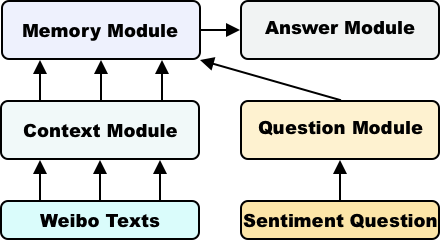
\includegraphics[width=0.4\textwidth]{TF-MN.png}
	\centering
	\caption{The architecture diagram of TF-MN.}\label{TF-MN}
\end{figure}

\bibliographystyle{IEEEtran}
\bibliography{ref.bib}
\EOD
\end{document}
